\documentclass[unicode,11pt,a4paper,oneside,numbers=endperiod,openany]{scrartcl}

\usepackage{graphicx}
\usepackage{subcaption}
\usepackage{auto-pst-pdf}
\graphicspath{/home/sklampt/ETH/fs21/hpclab/hpclab_euler/Project1/membench/}

\input{assignment.sty}
\begin{document}


\setassignment
\setduedate{09.03.2020 (midnight)}

\serieheader{High-Performance Computing Lab for CSE}{2020}{Student: Sina Klampt}{Discussed with: Alain Hügli, Anna Hutter}{Solution for Project 1}{}
\newline

\assignmentpolicy
In this project you will practice memory access optimization, performance-oriented programming, and OpenMP parallelizaton 
on Euler.

\section{Explaining Memory Hierarchies \punkte{30}}

\subsection{Identifying Parameters}
Using the commands given on the exercise sheet, I was able to find the following values for the memory hierarchy on the computer node of the Euler cluster:
\begin{center}
    \begin{tabular}{ |l|l| }
    \hline
    Main memory & 32 GB \\ \hline
    L3 cache & 6 MB \\ \hline
    L2 cache & 256 kB \\ \hline
    L1 cache & 32 kB \\
    \hline
    \end{tabular}
\end{center}

\subsection{Running Membench}
In this exercise we were supposed to run the membench program on our local machine and on the Euler cluster.

The first plot (Fig. 1) represents the results on my local machine. I have a Intel Core i7 processor with 16 GB of Main Memory, 196 kB of L1 cache, 2 MB of L2 cache and 8 MB of L3 cache.

The second plot (Fig. 2) represents the results using Euler. I have used the Xeon Gold 6150 CPU.
When we look at the time axis, we can easily see that the performance of the Euler cluster is much better than on my local machine.
\begin{figure}[h!]
    \centering
    \includegraphics{../membench/generic.ps}
    \caption{Plot for local machine}
\end{figure}
\begin{figure}[h!]
    \centering
    \includegraphics{generic_euler.ps}
    \caption{Plot for Euler}
\end{figure}

\subsection{Memory Access Patterns}
In the first case we had: csize = 128 and stride = 1. Since one integer corresponds to 4 Bytes, we have 128 times 4 which equals 512. Thus we need to look at the red line corresponding to 0.5 kB.

In the second case we had: csize = 

\subsection{Temporal Locality}
asdf


\section{Optimize Square Matrix-Matrix Multiplication  \punkte{70}}

\end{document}
